\vspace*{-0.5cm}
Le câblage du cryostat consiste en deux parties: 
\paragraph*{Les câbles DC: }ils véhiculent les signaux continus. Au nombre de 17, ils sont thermalisés à chaque étage pour limiter le bruit thermique.
\paragraph*{Les câbles coaxiaux: }les deux grilles rapides, le signal d'entrée et le signal de sortie. Ils font l'objet de beaucoup d'attention, afin d'avoir les meilleures mesures possibles.

\vspace*{0.8cm}
\begin{figure}[h]
    \begin{center}
        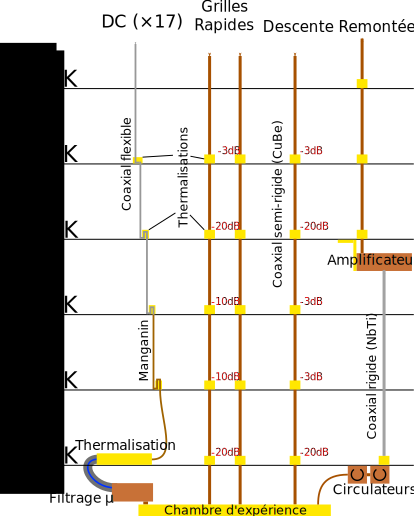
\includegraphics[width=0.7\textwidth]{Images/Cablage_schema}
        \caption{Schéma de câblage de l'expérience}
        \label{cablage_schema}
    \end{center}
\end{figure}




\section{Choix des matériaux}
Parlons tout d'abord des câbles de descente. Ceux-ci véhiculent le bruit thermique d'étage en étage, ce que nous voulons limiter au maximum.

Nous faisons donc le choix de câbles atténuant le signal afin de limiter l'apport de bruit. Ceci permet en plus de limiter les ponts thermiques entre étages dûs à la conductivité des câbles.
\newline

Les câbles DC sont alors:
\begin{itemize}
    \item des câbles coaxiaux souples entre 300K et 800mK, peu résistifs (le signal est suffisant pour avoir un bon rapport signal/bruit)
    \item des câbles de Manganin, très résistifs ($\sim45\Omega/m$), jusqu'à 20mK (l'étage le plus froid)
    \item des câbles peu résistifs ($\sim0.4\Omega/m$) jusqu'à la chambre d'expérience
    \newline
\end{itemize}

et les câbles RF coaxiaux semi-rigides de descente sont:
\begin{itemize}
    \item en Cuivre-Béryllium, thermalisé à chaque étage, jusqu'à 20mK. Le CuBe est beaucoup plus résistif que le Cuivre.
    \item en Cuivre jusqu'à la chambre d'expérience
\end{itemize}

Les câbles sont cintrés en "U" entre chaque étage, afin de limiter le passage des radiations au maximum. Ceci permet de plus d'avoir une certaine souplesse dans les câbles pour les connecter sans trop de difficultés.\newline

Enfin, on rajoute à chaque étage un atténuateur (valeur en rouge sur le schéma). Ceci permet d'envoyer en amont du cryostat un signal très fort, qui détruirait les échantillons, pour avoir dès le départ un rapport signal/bruit très bon.


\paragraph*{Pour le câble de remontée,}on raisonne différemment: il faut atténuer le signal le moins possible, jusqu'à l'amplificateur haute fréquence qui est situé à 4K (sa température nominale de fonctionnement). Un câble rigide de Niobium-Titane est alors utilisé.

Afin de limiter le "retour" de signal de l'amplificateur par ce câble, on thermalise deux circulateurs à 20mK. On utilise des câbles de Cuivre pour les connexions avec la chambre d'expérience.





%\section{Principe des câbles coaxiaux}
\section{Thermalisation électronique}
Une grande partie du bruit provient de la température électronique. Si les câbles ne sont pas bien thermalisés, on risque de ne mesurer qu'un bruit à 300K.\newline

Les câbles coaxiaux sont thermalisés à chaque étage du cryostat par des pinces, reliées par des câbles de cuivre jusqu'aux platines du cryostat. L'ensemble des pièces est bien sûr doré pour avoir les meilleurs contacts thermiques possibles ; les pores des parois en contact sont bouchées par de l'Apiezon N, à l'instar de la pâte thermique de nos processeurs.
\newline

Les câbles DC sont thermalisés à chaque étage par des presses dorées grâce à de la Stycast. Cette époxy permet une très bonne thermalisation des câbles fins aux presses dorées et montées sur les platines du cryostat.

Une thermalisation s'effectue aussi au niveau du boîtier de thermalisation où les câbles font des méandres afin d'assurer une bonne thermalisation électronique.

\begin{figure*}
    \centering
    \begin{subfigure}[t]{0.5\textwidth}
        \centering
        \includegraphics[height=1.2\textwidth]{Images/Thermalisation/DC}
        \caption{Fils de Manganin "stycastés" dans une presse dorée}
    \end{subfigure}%
    ~ 
    \begin{subfigure}[t]{0.5\textwidth}
        \centering
        \includegraphics[height=1.2\textwidth]{Images/Thermalisation/Coax}
        \caption{Câbles coaxiaux thermalisés}
    \end{subfigure}
    \caption{Thermalisation des câbles sur la platine du cryostat}
\end{figure*}

\newpage
\section{Filtrage des lignes DC}
En plus de la thermalisation, les lignes DC sont filtrées à l'étage 20mK. Un premier filtrage est effectué dans le boîtier de thermalisation à l'aide d'un filtre Passe-Bas RC du second ordre.

\begin{figure}[h]
    \begin{center}
        \includegraphics[height=0.4\textwidth]{Images/Thermalisation/DC3}
        \caption{Boîtier de thermalisation non soudé}
        \label{coax_denudage}
    \end{center}
\end{figure}

Un second filtrage est effectué grâce à l'Eccosorb. Cette résine composite à base d'époxy (même fabricant que la Stycast, mêmes solutions) absorbe très efficacement les micro-ondes résultant du bruit électronique.

Il a donc fallu mettre en place un petit boîtier, dans lequel nous faisons passer 17 câbles bleus de 80cm, compartimenté pour que l'Eccosorb n'abîme pas les prises lors du durcissement et des cycles de refroidissement.

J'ai donc décidé de dessiner des pièces en 3D sous OpenSCAD afin de former ces compartiments. Après quelques recherches, il est apparu que le matériau le plus utilisé en impression 3D, le PLA, peut être utilisé dans un cryostat (bien que jamais utilisé jusqu'ici).\newline

En fait, beaucoup de matériaux ne sont pas compatibles avec de telles applications. Notamment, la faible pression dans le cryostat peut faire dégazer les matériaux (air dans les parois poreuses, ou des composants du matériau lui-même qui s'évapore). La plupart des matériaux élastiques sont dans ce cas.

De plus, certains matériaux peuvent ne pas supporter les cycles de refroidissement dans le cryostat. C'était le cas des précédentes séparations, qui ont alors cassé les câbles qui passaient au travers.

\subsection{Blindage des câbles coaxiaux}
En aval du boîtier de thermalisation, les câbles sont bien thermalisés et déjà bien filtrés. On ne voudrait donc pas laisser les câbles DC non blindés, au risque de recevoir des radiations, ne serait-ce que de l'étage à 100mK.

Une tresse métallique soudée à la masse entoure donc les câbles jusqu'au boîtier de filtrage micro-ondes. Celui-ci est directement branché sur la chambre d'expérience, les câbles restent donc isolés.

\begin{figure*}[t!]
    \centering
    \begin{subfigure}[t]{0.6\textwidth}
        \centering
        \includegraphics[height=0.633\textwidth]{Images/Thermalisation/Filtrage3D}
        \caption{Modélisation 3D des pièces dans le boîtier}
    \end{subfigure}%
    ~ 
    \begin{subfigure}[t]{0.4\textwidth}
        \centering
        \includegraphics[height=0.95\textwidth]{Images/Thermalisation/Filtrage}
        \caption{Boîtier de filtrage en place dans le cryostat}
    \end{subfigure}
    \caption{Boîtier de filtrage, rempli d'Eccosorb}
\end{figure*}






\section{Fabrication des câbles coaxiaux}
Comme je l'ai précisé plus haut, les signaux RF sont véhiculés par des câbles coaxiaux semi-rigides.

J'ai donc procédé intégralement à la fabrication et la caractérisation de ces câbles.

La moindre imperfection des câbles coaxiaux se ressent fortement sur leur atténuation -- nous verrons cela plus tard -- , il faut donc les manier et les cintrer en faisant attention à ne pas les tordre.

\paragraph*{Dénudage} Il faut dénuder quelques millimètres du câble pour souder la pin sur l’âme du
câble coaxial. On utilisera le support 21B ainsi que la petite scie. Il faut aller doucement
sans appuyer, jusqu’à ce qu’on sente que c’est "lisse".
\begin{figure}[h]
    \begin{center}
        \includegraphics[height=0.48\textwidth]{Images/Coax/1}
        \quad
        \includegraphics[height=0.48\textwidth]{Images/Coax/2}
        \caption{Dénudage d'un câble coaxial}
        \label{coax_denudage}
    \end{center}
\end{figure}

\paragraph*{Soudure de la pin centrale} On fixe la pin sur l’âme du câble, puis on serre le tout en
place avec la pièce W60 Il ne faut pas oublier l’entretoise W56 entre la pin et l’isolant
encore en place.
Pour souder il suffit de chauffer l’extérieur de la pin tout en positionnant le fil d’étain sur
le trou sur le bord de la pin.
\begin{figure}[h]
    \begin{center}
        \includegraphics[width=0.60\textwidth]{Images/Coax/3}
        \caption{Pin centrale soudée sur le câble}
        \label{coax_soudure_centre}
    \end{center}
\end{figure}

\paragraph*{Soudure de la prise extérieur} On fixe sur la prise mâle une prise femelle factice W14M
(81) qui permet de positionner comme il faut la prise. Comme à l’étape précédente on
serre le tout en place.
Le plus efficace est de faire un tortillon d’étain au-dessus de la prise, que l’on chauffe. En
étant un peu patient l’étain va fondre et rentrer naturellement dans la prise.
\begin{figure}[h]
    \begin{center}
        \includegraphics[height=0.48\textwidth]{Images/Coax/4}
        \quad
        \includegraphics[height=0.48\textwidth]{Images/Coax/5}
        \caption{Soudure de la prise extérieure}
        \label{coax_soudure_exterieur}
    \end{center}
\end{figure}

\paragraph*{Fixation de l’isolant}  La dernière étape est de mettre l’isolant entre la prise et la pin. on
utilise la pièce W52 (W53) que l’on serre à la clé dynamométrique. On place l’isolant à
l’intérieur, et on pousse d’un coup avec la pièce complémentaire.
Mesure du câble nécessaire Maintenant il faut prendre la dimension de câble à couper.
Sur le montage il faut prendre la dimension entre les deux{}
\begin{figure}[h]
    \begin{center}
        \includegraphics[width=0.60\textwidth]{Images/Coax/6}
        \caption{Fixation de l’isolant}
        \label{coax_fixation_isolant}
    \end{center}
\end{figure}








\newpage
\section{Caractérisation des câbles coaxiaux}

Maintenant que les câbles ont été cintrés et connectorisés, il faut mesurer leur caractéristique atténuation/fréquence. D'une part pour vérifier si les câbles sont utilisables, et d'autre part pour avoir les valeurs exactes d'atténuation afin de calibrer nos mesures à fréquence fixée.

L'appareil dédié à cette tâche est le VNA (Vector Network Analyzer) ou PNA (Performance Network Analyzer). L'équipe a récemment fait l'acquisition d'un PNA N5242 de Agilent.

\begin{figure}[h]
    \begin{center}
        \includegraphics[width=0.65\textwidth]{Images/VNA}
        \caption{Le PNA de l'équipe}
        \label{PNA}
    \end{center}
\end{figure}

En se plaçant sur un canal de mesure, on calibre l'appareil avec les câbles flexibles supplémentaires, puis on connecte notre câble coaxial.

\begin{figure}
    \begin{center}
        \includegraphics[width=0.65\textwidth]{Images/Caracs/abime2.png}
        \caption{La caractéristique d'un câble correct(vert) et un abîmé (violet)}
        \label{Carac1}
    \end{center}
\end{figure}
